\chapter{Stand der Technik}
\label{chap:technikStand}
%\section{Theorien}
%\section{Techniken}
    Zur Analyse des aktuellen Standes der Technik und Forschung in Bezug zur Konzeption von Software-Lösungen, mit denen 
    die formalisierten Interaktionen der Softwareentwickler vereinfacht werden können, erfolgt in diesem 
    Kapitel ein systematisches Literaturreview. Die Literaturprüfung wird gemäß den Richtlinien, die in der Publikation 
    von \cite{Kitchenham2007} vorgeschlagen werden, durchgeführt. 

    %\section{Methodiken}
    %\label{sec:methodiken}
    %    Im Rahmen dieser Arbeit wurden zur Informationserhebung zuerst ein systematisches Literaturreview durchgeführt und

    \section{Systematisches Literaturreview}
    \label{subsec:systematischesLiteraturReview}
        Die Thematik des systematischen Literaturreviews wurde bereits in den einleitenden Kapiteln erwähnt. 
        Dieser Abschnitt widmet sich ausschließlich der Anwendung der Richtlinien und dem daraus abgeleiteten Stand der Technik 
        abhängig zu dem in der Arbeit behandelten Thema. 

    \subsection{Ziele des Systematischen Literaturreviews}
        Das Ziel dieses systematischen Literaturreviews ist es, die aktuellen Fortschritte von Smart Home Plattformen und 
        Gateways in Richtung der entwicklerseitigen Benutzerfreundlichkeit zu recherchieren. Dabei liegt der Schwerpunkt 
        auf der Usability und der einfachen Handhabung der formalisierten Interaktionen der Softwareentwickler. Es gilt zu 
        analysieren, ob es in diesem Themenbereich bereits Publikationen und Forschungen gibt und welche Entscheidungen 
        getroffen werden müssen, um die Weiterentwicklung eines Systems nicht je nach hinzukommender Funktionalität oder 
        auch Bedingung komplexer werden zu lassen. Die Ergebnisse dieses systematischen Literaturreviews sollen daraufhin 
        als Grundlage der Konzeption einer solchen Plattform dienen und mit einfließen. 

    \subsection{Suchstrategie- und anfragen}
        Dieser Abschnitt beschreibt die Suchstrategie und die Anfragen zu dem systematischen Literaturreview. Hierbei wird 
        erläutert, anhand welcher Kriterien die Literatur ausgewählt wird.
        \\
        In den ersten Schritten werden anhand der Forschungsfragen in Kapitel (\ref{sec:forschungsfragen}) die Stichpunkte 
        aufgegriffen und als Suchterm formuliert. Die daraus resultierenden Suchterme, die der tabellarischen Darstellung 
        (\ref{tab:slr}) zu entnehmen sind, werden in diversen wissenschaftlichen Fachdatenbanken recherchiert und analysiert. 
        Die Ergebnisse werden nach ihrem Titel und der Zusammenfassung sortiert. Gibt es Publikationen mit vergleichbaren 
        Inhalten, so sind diese in weiteren Schritten näher zu betrachten. Damit die Literaturrecherche weitere Ergebnisse 
        erzielt, wird beim studieren der Publikationen die Schneeballsuche angewendet. Dabei wird in den Quellen der jeweiligen 
        Literatur auf weitere Verweise geschaut, die ebenso potentielle Inhalte bearbeiten. Die Kombination beider 
        Literaturergebnisse bilden die Grundlage der zu analysierenden Quellen und geben so den Stand der Technik wieder.
        \begin{figure}[hbt!]
            \centering
            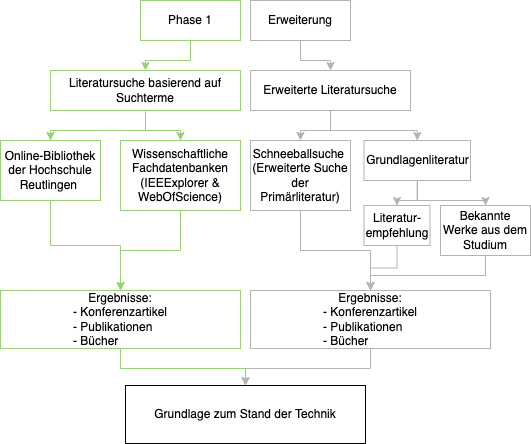
\includegraphics[width=13cm,height=13cm,keepaspectratio]{images/slr_walkthrough.png}
            \caption{Strategie der Literatursuche}
            \label{fig:slr}
        \end{figure}
        \\
        Die generierten Suchterme, die daraus resultierenden Literaturergebnisse und der damit einhergehende Suchverlauf ist 
        zur Nachvollziehbarkeit tabellarisch aufgeführt:
        \\
        \linebreak
        \pagebreak
        \begin{table}[hbt!]
            \begin{center}
                \begin{tabular}{| p{2.9cm} | p{1.9cm} | p{1.6cm} | p{1.9cm} | p{1.9cm} | p{1.8cm} | p{1.8cm} | }
                    \hline
                        \textbf{Suchanfrage} & \textbf{Datum} & \textbf{Filter} & \textbf{Plattform} & \textbf{Ergebnisse} & \textbf{Gesehene} & \textbf{Relevant} \\
                    % \hline
                        % formalized interactions software development & 08.04.2022, 03.05.2022 & Nein & IEEExplorer, WebOfScience & 55, 106 & 5, 4 & 0, 0 \\ 
                    \hline
                        formalized interactions software development architecture  & 11.04.2022, 03.05.2022 & Nein & IEEExplorer, WebOfScience & 13, 26 & 6, 4 & 0, 0 \\ 
                    \hline
                        usability AND formalized interactions AND architecture & 11.04.2022, 03.05.2022 & Nein & IEEExplorer, WebOfScience & 3, 7 & 1, 3 & 0, 1 \\ % A Conceptual Model of Service Customization and Its Implementation
                    \hline
                        usability AND formalized interactions AND architecture AND smart home & 01.05.2022 & Nein & IEEExplorer, WebOfScience & 0, 0 & 0, 0 & 0, 0 \\
                    \hline
                        usability AND formalized interactions AND software development AND architecture & 02.05.2022 & Nein & IEEExplorer, WebOfScience & 1, 1 & 1, 1 & 0, 1 \\
                    \hline
                    %    usability AND formalized interactions AND software development AND architecture AND smart home & 02.05.2022, 03.05.2022 & Nein & IEEExplorer, WebOfScience & 0, 0 & 0, 0 & 0, 0 \\
                    %\hline
                        usability AND architecture AND gateway AND smart home & 06.05.2022 & Nein & IEEExplorer, WebOfScience & 2, 4 & 1, 1 & 1, 1 \\
                    \hline
                        usability AND formalized interaction AND (architecture OR smart home OR software developer OR gateway) & 09.05.2022 & Nein & IEEExplorer, WebOfScience & 3, 10 & 1, 2 & 0, 0 \\
                    \hline
                        usability AND architecture AND smart home AND (formalized interaction OR software developer OR iot) & 09.05.2022 & Nein & IEEExplorer, WebOfScience & 13, 22 & 3, 3 & 0, 0 \\
                    \hline
                \end{tabular}
            \end{center}
            \caption{Suchprotokoll des Systematischen Literaturreviews}
            \label{tab:slr}
        \end{table}
    \subsection{Datenextraktion und Synthese}
        Zu der zielgerichteten Datenextraktion werden in Anlehnung an die Richtlinien des systematischen Literaturreviews die folgenden 
        Einschluss- und Ausschlusskriterien definiert, die dabei helfen, die relevanten Publikationen zu finden:
        \begin{table}[hbt!]
            \centering
            \begin{tabular}{p{0.125cm} p{15cm}}
                    \textbf{\#} & \textbf{Einschluss-Kriterien}\\ 
                \hline
                    1  & Die Literatur ist in den wissenschaftlichen Fachdatenbanken veröffentlicht, darunter: WebOfScience, IEEExplorer, SpringerLink, Elsevier, Addison-Wesley, dpunkt-Verlag, ACM und Google Scholar  \\ 
                \hline
                    2  & Der Beitrag wurde nach 2010 veröffentlicht \\ 
                \hline
                    3  & Die Veröffentlichung ist in deutscher oder englischer Sprache \\
                \hline
                    \textbf{\#} & \textbf{Ausschluss-Kriterien}\\ 
                \hline
                    1  & Die Veröffentlichung beinhaltet, bzw. behandelt nicht die Schlagworte usability, architecture, formalized interaction oder iot \\ 
                \hline
                    2  & Die Publikation gehört zu der Literatur der Grauzone \\ 
                \hline
                    3  & Die Veröffentlichung hat weniger als 5 Zitationen \\
                \hline
                    4  & Die Literatur hat weniger als 5 Seiten Inhalt \\
            \end{tabular}
            \caption{Einschluss- und Ausschlusskriterien des systematischen Literaturreviews}
            \label{tab:slr_criteria}
        \end{table}
        \\
        Mit der Forschungsfrage, den Suchtermen und den Einschluss- und Ausschlusskriterien zu der Quellenrecherche werden während der Anwendung
        des systematischen Literaturreview-Templates und deren Richtlinien die erzielten Ergebnisse synthetisiert und zusammengefasst. Im Rahmen 
        dieser Forschungsfrage und der Auslegung der Suchterme, die in Tabelle (\ref{tab:slr}) zu entnehmen sind, ergab sich nicht die Menge an Literatur, 
        die notwendig ist, um ein umfangreiches Literaturreview im Stil des Templates durchzuführen. Demnach ist kein vollständiges systematisches Literaturreview 
        möglich. Die wenigen relevanten Ergebnisse des Literaturreviews geben einen Einblick in Bereiche, die als Gedankenanstoß und zum transferieren von 
        Wissen, Gedanken und Ideen geeignet sind. 
        \\
        \linebreak
        Unter der Betrachtung des Resultats des durchgeführten Literaturreviews gilt die Forschungsfrage als innovativ und eröffnet eine 
        neue Sichtweise basierend auf der Literatur. Um dennoch eine fundierte wissenschaftliche Grundlage zu repräsentieren, wird in 
        folgendem Abschnitt auf Referenzen und Literatur eingegangen, die Teile der Forschungsfrage abdecken und mehr als Gedankenanstoß 
        anzusehen sind, beziehungsweise auch einen partiellen Einblick in den Stand der Technik bieten. 

\section{Zusammenfassung} 
    Speziell auf die Forschungsfrage in Kapitel (\ref{sec:forschungsfragen}) gibt es in dem heutigen Stand der Technik keine explizite 
    Literatur, welche den Gedanken aufgreift und behandelt. Die Literatur, die bei dem systematischen Literaturrecherche erarbeitet wurde, 
    deckt trotz dessen manche Aspekten ab, die interessante Anhaltspunkte und Ideen thematisieren. Diese geben Impulse und helfen bei den weiteren 
    Schritten in dieser Arbeit hinsichtlich der Konzeption. 
    \\
    
    \subsection{Publikationen}
    \label{subsec:publications}
        Im Folgenden wird die relevante Literatur aufgegriffen und zusammengefasst, sodass ein Einblick in den Prozess der 
        Informationserhebung, der Sammlung von Erfahrungswerten und Ideen gewährleistet wird.
        
        \subsubsection*{Design and Realization of a Framework for Human-System Interaction in Smart Homes}
            In dem Artikel von \cite{Wu2012} wird zu Anfang die Beziehung zwischen Benutzern, Räumlichkeiten und 
            Diensten analysiert. Basierend auf den daraus gewonnenen Erkenntnissen wird ein Framework und ein 
            entsprechender Algorithmus entwickelt, welcher die Interaktionsbeziehungen modelliert. Basierend auf den  
            Ergebnissen wird ein Framework entwickelt, welches die Interaktionsanforderungen abdeckt. Hauptmerkmale 
            waren dabei Komfort, Bequemlichkeit und Sicherheit. Zur abschließenden Überprüfung des Designkonzeptes und 
            der Implementierung wurden Probanden zum Testen der Anwendung ausgewählt und anschließend ein Interview 
            durchgeführt. Das Evaluierungsergebnis zeigt, dass das Framework eine gute Einführung in die Verbesserung 
            der Mensch-System-Interaktionen darstellt. 

        \subsubsection*{Seamless Integration of Heterogeneous Devices and Access Control in Smart Homes}
            Der Artikel von \cite{Kim2012} erarbeitet einen Vorschlag einer ganzheitlichen und erweiterbaren 
            Softwarearchitektur, welches Dienste und heterogene protokoll- und herstellerspezifische Geräte 
            nahtlos integrieren lässt und Sicherheit über das Internet gewährleistet. Grundlegend wird hierbei auf das 
            \acs{OSGI} Framework gesetzt. Dadurch wird die semantische Interoperabilität hervorgehoben. Dies ist die Fähigkeit, 
            neue Anwendungen und Treiber zur Laufzeit in das bereitgestellte System zu integrieren \cite{Kim2012}. 
            Zusätzlich zu dem System wird im Rahmen dieser Publikation ein Zugangskontrollmodell für spezielle \acl{SH} 
            Szenarien integriert. Zur Beweisführung wird das Konzept anhand von semantischen Erkennungen von Heimgeräten zur 
            Laufzeit demonstriert. Dafür werden mehrere Protokolle, darunter X10, ZigBee und Insteon, in einen realen Test 
            integriert. Die Arbeit behandelt die folgenden Schwerpunkte \cite{Kim2012}:
            \begin{enumerate}
                \item Analyse einer Reihe von Heimnetzprotokollen hinsichtlich ihrer Erkennungs- und Integrationsanforderungen.
                \item Eine erweiterbare Home-Gateway-Architektur, die es ermöglicht, heterogene Geräte während der Laufzeit flexibel zu installieren, zu verwalten und darauf zuzugreifen.
                \item Ein neuartiger Zugangskontrollmechanismus speziell für Smart-Home-Systeme.
                \item Die Umsetzung des vorgeschlagenen Konzepts, indem gezeigt wird, wie verschiedene Geräte integriert und von Endbenutzern aufgerufen werden können.
            \end{enumerate}
            Die Architektur und die damit eingesetzte semantische Abstraktionsschicht unterstützt laut den Ergebnisse 
            erheblich die Anwendungsentwicklung. 
            \\
            Mit der Zugriffskontrollrichtlinie wird den Hausbesitzern eine stabile Kontrolle darüber gegeben, mit der 
            die Benutzer auf die smarte Geräte zugreifen können. Das Resultat dieser Arbeit scheint zu zeigen, dass damit 
            die Barriere für \acl{SH} Systeme gesenkt wird. 

        \subsubsection*{Wireless Architectures for Heterogeneous Sensing in Smart Home Applications: Concepts and Real Implementation}
            %In diesem Beitrag wurden aktuelle Trends bei der Nutzung drahtloser Architekturen für Smart-Home-Anwendungen 
            %diskutiert. Die in Smart Homes üblicherweise eingesetzten drahtlosen Technologien wurden berücksichtigt und WSNs 
            %wurden als geeignetes architektonisches Werkzeug zur Implementierung der In-Home-Überwachung analysiert. Unter 
            %den Smart-Home-Funktionalitäten wurden verteilte Smart Metering und Seniorenhilfe als zwei repräsentative 
            %Beispiele angesehen, die die Einführung von Smart-Home-Drahtlossystemen vorantreiben können. Tatsächlich sind 
            %sowohl Energieeinsparung als auch die Reduzierung von Gesundheitskosten von besonderem Interesse in einer Welt, in 
            %der die Energieressourcen zur Neige gehen und die Bevölkerung schnell altert.
            %Die Vorteile, die sich aus der Verwendung drahtloser Architekturen ergeben, wurden analysiert, wobei der 
            %Schwerpunkt auf der Schätzung des Benutzerverhaltens lag. Spezielle Methoden zur Bewertung der täglichen 
            %Aktivitäten wurden untersucht und in die vorgeschlagene drahtlose Architektur zur Benutzerüberwachung und 
            %-lokalisierung integriert. Nichtinvasive drahtlose Lösungen, die die elektromagnetische Erfassung und die weit 
            %verbreiteten mobilen Geräte wie Smartphones nutzen, wurden eingeführt. Die opportunistische Nutzung bereits 
            %verfügbarer Informationen, die durch elektromagnetische Feldstörungen bereitgestellt werden, wurde 
            %vorgeschlagen, um zwei wichtige Eckpunkte des zukünftigen Smart Home zu gewährleisten: Benutzerakzeptanz und 
            %geringe Systemkomplexität. Einige repräsentative Ergebnisse der laufenden Aktivitäten am ELEDIA Research Center 
            %am Department of Information Engineering and Computer Science (DISI), University of Trento, Trento, Italien, 
            %wurden berichtet, um Beispiele für die Potenziale einer opportunistischen Nutzung drahtloser Technologien zu 
            %liefern sind bereits Teil unseres eigentlichen Alltags.

        \subsubsection*{My House, My Rules: A Private-by-Design Smart Home Platform}
            %Die Smart-Home-Technologie ist weit verbreitet. Mehrere Fälle von massiver Unternehmensüberwachung und Episoden 
            %von Verletzungen von Sensordaten haben jedoch viele Datenschutzbedenken bei potenziellen Verbrauchern geweckt. 
            %Dieses Whitepaper stellt PatrIoT vor, eine Private-by-Design-IoT-Plattform für Smart-Home-Umgebungen. PatrIoT 
            %überarbeitet die typische Architektur bestehender IoT-Plattformen und bietet ein alternatives Design, bei dem der 
            %Hausbesitzer die volle Eigentümerschaft und Kontrolle über die von intelligenten Geräten generierten Daten behält. 
            %Es nutzt Intel SGX, um den unbefugten Zugriff auf die Daten durch nicht vertrauenswürdige IoT-Cloud-Anbieter zu 
            %verhindern, und bietet Hausbesitzern eine intuitive Sicherheitsabstraktion namens Flowwall, mit der sie 
            %benutzerfreundliche Richtlinien zur Steuerung sensibler Sensordatenflüsse in ihren Smart Homes festlegen können. 
            %Wir haben einen PatrIoT-Prototypen gebaut und evaluiert. Die meisten Teilnehmer einer Feldstudie hielten 
            %PatrIoT für benutzerfreundlich und die unterstützten Richtlinien für nützlich, um ihre Privatsphäre zu schützen.

            %Wir haben PatrIoT vorgestellt, eine Private-by-Design-IoT-Plattform, die eine sichere Datenverarbeitung durch die 
            %Nutzung sicherer Enklaven von SGX gewährleistet. Der Flowwall-Sicherheitsmonitor von PatrIoT ermöglicht 
            %Endbenutzern eine feinkörnige Kontrolle der von IoT-Geräten generierten Datenflüsse und verhindert potenzielle 
            %Datenschutzverletzungen durch die Durchsetzung einer Datenschutzrichtlinie.

        \subsubsection*{Fast-prototyping Approach to Design and Validate Architectures for Smart Home}  
            %Aufgrund der kontinuierlichen Entwicklung und Kommerzialisierung neuer IoT-Geräte für den Smart-Home-Kontext 
            %ändern sich die Anforderungen der Benutzer ständig und die Community benötigt schnelle Prototyping-Lösungen, um 
            %auf solche schnellen Notwendigkeiten vorbereitet zu sein. Dieses Papier zeigte, wie es möglich ist, ein komplexes 
            %Smart-Home-System zu entwickeln, das Funktionen implementiert, die aus einer soliden und aktuellen Studie über 
            %Benutzeranforderungen in Smart Homes extrahiert wurden, und zwar durch einige bekannte 
            %Fast-Prototyping-Plattformen und -Technologien wie Node-RED, IBM Watson, Telegram, Raspberry Pi 4 und das 
            %gesicherte MQTT-Protokoll. Ein laufendes Szenario wurde sowohl beim Design als auch bei der Entwicklung einer 
            %Referenzarchitektur verwendet und schließlich dazu genutzt, die Wirksamkeit der vorgeschlagenen Lösungen zu 
            %demonstrieren. Durch die entwickelte Infrastruktur können Benutzer tatsächlich die Aktionen ausführen, die für 
            %die betrachtete Literatur die wichtigsten für Menschen sind, wie z Beleuchtung steuern, c) Energie sparen dank 
            %eines autonomen Lichtmanagementsystems, das auf der Überwachung der Benutzerbewegungen basiert, d) das Haus über 
            %spezielle Webcams fernüberwachen, e) im Gefahrenfall Warnmeldungen generieren. Das durchgeführte Experiment kann 
            %als Inspiration für zukünftige Arbeiten genutzt werden, die innovative schnelle Prototyping-Lösungen vorschlagen 
            %würden. Aufgrund ihrer Ähnlichkeiten in Bezug auf die Notwendigkeiten und die Tendenz, praktische Arbeit für ihre 
            %Zwecke zu nutzen, können sowohl der Forschungs- als auch der Bildungsbereich von einer solchen Arbeit profitieren.
            

        % ggfs. auch kurz teasern, welche Plattformen aktuell auf dem Markt sind, bzw. kommerziell und nicht-kommerziell